\section{Modelling the Instruction Set in B}
% \begin{frame}
%   \frametitle{Modelling  Microcontrollers}  
% 
%   \begin{itemize}[<+->]
%   \item Relations 
%   \begin{itemize}
%   	\item States of platform  $\Leftrightarrow$ States of modell
% 		\begin{itemize}
% 		\item Registers and Memory $\Leftrightarrow$  Variables of model
% 		\end{itemize}
% 	\item Assembly Instructions $\Leftrightarrow$ B operations
%         \begin{itemize}
%         \item Changes of states of platform $\Leftrightarrow$ B substitutions
%         \end{itemize}
%   \end{itemize}
%     
%  \end{itemize}
% \end{frame}


\begin{frame}
 \frametitle{Structure of B Projects}
 \begin{center}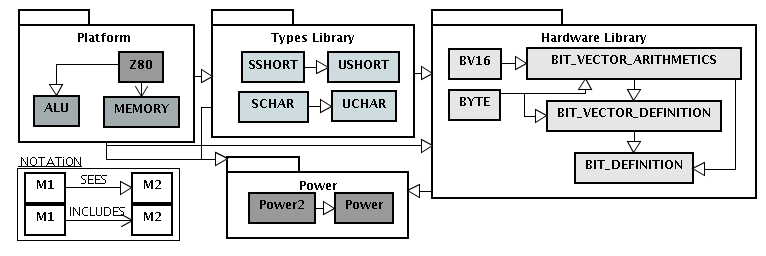
\includegraphics[width=1.\textwidth]{figures/diagramaEstrutural_vertical.png}
 \end{center}

 \end{frame}

 

 
\begin{frame}
 \frametitle{Hardware Library Project}

  	  	\begin{itemize}
 			\item The module \textit{BIT\_DEFINITION} has:
 			\begin{itemize}
                 
  	  		\item Definition of \textit{Bit}\\
  			{\small
 			$
 			\begin{array}{l}
 			\mathit{BIT} = 0..1 \\
 			\end{array}
 			$
 			}
 
 			\item The function $\mathit{bit\_not}$ is a unary function:
			{\small
			$
			\begin{array}{l}
			\mathit{bit\_not}  \in  \mathit{BIT}  \fun  \mathit{BIT}  \land \\
			\forall (\mathit{bb}).(\mathit{bb} \in \mathit{BIT} \implies \mathit{bit\_not}(\mathit{bb}) = 1-\mathit{bb})\\
			\end{array}
			$
			}

			\item Some utils lemmas to development proofs

			{\small
			$
			\begin{array}{l}
			\mathit{bit\_not}(0) = 1; 	\mathit{bit\_not}(1) = 0; \\
			\forall (\mathit{bb}).(\mathit{bb} \in \mathit{BIT} \implies \mathit{bit\_not}(\mathit{bit\_not}(\mathit{bb})) = \mathit{bb});
			\end{array}
			$
			}
			

			\end{itemize}
  		\end{itemize}


\end{frame}


 
 
\begin{frame}
 \frametitle{Hardware Library Project}

 	\begin{itemize}
 	  		\item The module \textit{BIT\_DEFINITION} also has:
 	  		\begin{itemize}
            \item The conjunction is a binary function defined as:
			{\small
			$
			\begin{array}{l}
			\mathit{bit\_and} \in \mathit{BIT} \times \mathit{BIT} \fun \mathit{BIT} \land \\
			\forall (\mathit{b1}, \mathit{b2}).(\mathit{b1}  \in \mathit{BIT}  \land \mathit{b2} \in \mathit{BIT} \implies \\
			\quad ((\mathit{bit\_and}(\mathit{b1}, \mathit{b2}) = 1) \iff (\mathit{b1} =1)  \land  (\mathit{b2} = 1))) \land \\
			 bit\_and(0,0) = 0	\land bit\_and(0,1) = 0	\land\\
			 bit\_and(1,0) = 0	\land bit\_and(1,1) = 1 \\
			\end{array}
			$
			}
 	  		\item Definions of 	$\mathit{bit\_or},\mathit{bit\_xor}$ and
 	  		$bool\_to\_bit$.
 	  		\item Lemmas for associativity and commutativity of functions
           \end{itemize}



           
 	\end{itemize}


\end{frame}


\begin{frame}
 \frametitle{Hardware Library Project}

 	\begin{itemize}
       \item  The module \textit{BIT\_VECTOR\_DEFINITION} has:

           \begin{itemize}
	 	  		\item Definition of bit vectors:
				{\small
				$
				\begin{array}{l}
				\mathit{BIT\_VECTOR} = \seq (\mathit{BIT}) % Implementa��o antiga, mas vale
				\end{array}
				$
				}
	 	  		\item Definition of functions:
	 	  		 {\small
	 	  		 	          
	          \it bv\_nat  $\in$  \it BIT\_VECTOR  $\fun$ $\nat$
	          $\land$ \\
	          \it bv\_nat \rm =  $\lambda$  \rm (\it bv\rm )\rm .\rm (\it bv 
	          $\in$  \it BIT\_VECTOR  $\mid$ \\ \rm (  $\sum$  \it idx \rm . \rm (\it idx  $\in$  \bf dom\rm (\it bv\rm )  $\mid$  \rm
	          (\rm 2$^{idx}$\rm )  $\times$  \it bv\rm (\it idx\rm )\rm )\rm )\rm )
			   
% 				$
% 				\begin{array}{l}
% 				\mathit{bv\_size} \in \mathit{BIT\_VECTOR} \fun \nat_1 \land \\
% 				\mathit{bv\_size} = \lambda bv \bullet (bv \in \mathit{BIT\_VECTOR} \mid \mathbf{size}(bv))
% 				\end{array}
% 				$
				}
				\item It has others functions: \textit{bv\_catenate}, \textit{bv\_sub},
				\textit{bv\_not}, \textit{bv\_and}, \textit{bv\_or}, \textit{bv\_xor},
				\textit{bv\_set}, \textit{bv\_clear} and \ldots
				\begin{itemize}
		                  \item These functions use the definitions of  \textit{BIT\_DEFINITION}
		              	\end{itemize}
	           \end{itemize}
		\item The module \textit{BIT\_VECTOR\_ARITHMETICS} define basics arithmetic functions
        \item The module \textit{BYTE} and \textit{BV16\_DEFINITION} define specialized functions for bit vectors of size 8 and 16
 	\end{itemize}

\end{frame}




\begin{frame}
 \frametitle{Types Library Project}
	  	\begin{itemize}
                    
	        \item Define the common types and functions on platforms of 8 and 16 bits
	        \item For example:
	        \begin{itemize}
	          \item Function: \it uchar\_schar $\in$ \it UCHAR $\fun$ \it SCHAR	  
				%\hspace*{0.0in} 
	%  		  \hspace*{0.0in}\it uchar\_schar\rm = $\lambda$ \rm (\it v1\rm )\rm .\rm (\it v1 $\in$ \it UCHAR
	%  			$\land$  \it v1 $\leq$ \it SCHAR\_MAX $\mid$  \it v1\rm )  $\land$\\
	%  			\hspace*{0.0in}\it uchar\_schar\rm = $\lambda$ \rm (\it v1\rm )\rm .\rm (\it v1 $\in$ \it UCHAR
	%  			$\land$   $\neg$ \rm (\it v1 $\leq$ \it SCHAR\_MAX\rm )  $\mid$  \it v1\rm -\it UCHAR\_MAX \rm + \rm 1
	%  			\rm )

	          \item Lemma: $\forall(x).( x \in UCHAR \Rightarrow
	          uchar\_schar(schar\_uchar(x)) = x)$
	        \end{itemize}
	      \end{itemize}
	
	\begin{table}[h]
	\begin{center}
	{\scriptsize
	\begin{tabular}{|c|c|c|c|c|c|c|}
	\hline
	 $Type$&$\mathit{UCHAR}$&$\mathit{SCHAR}$&$\mathit{USHORTINT}$&$\mathit{SSHORTINT}$&$\mathit{BYTE}$&$\mathit{BV16}$\\
	 \hline $Range$&0..255&-128..127&0..65.535&-32.768..32.767&--&--\\ \hline
	 $Size$ & 1 byte & 1 byte & 2 bytes & 2 bytes &  1 bytes & 2 bytes \\ \hline
	\end{tabular}
	}
	\end{center}
	\caption{Description of integer data types}
	\label{tab:types}
	\end{table}
\end{frame}

 
\begin{frame}
 \frametitle{Platform Project (Z80)}
  \begin{itemize}
    \item Z80 is a 8 bits microcontroller with 16 bits address space
    \item Supports:
    \begin{itemize}
      \item 158 instructions (included all of 8080 microcontroller )
      \item Several addressing modes and interruption types
      \item 256 input and output ports (8 bits)
      \item Some operations with 16 bits
    \end{itemize}

  
  \item Modelling 
  \begin{itemize}
  	\item States of platform  $\Leftrightarrow$ States of model
		\begin{itemize}
		\item Registers and Memory $\Leftrightarrow$  Variables of model
		\end{itemize}
	\item Assembly Instructions $\Leftrightarrow$ B operations
        \begin{itemize}
        \item Changes of states of platform $\Leftrightarrow$ B substitutions
        \end{itemize}
  
    
 \end{itemize}

      
  \end{itemize}

\end{frame}

\begin{frame}
\frametitle{Modelling Registers, Input/Output Ports and Instructions from Z80}
%  \begin{itemize}
%  \item Header of Modelling B
%  \end{itemize}  
	 {\scriptsize
	 \begin{sloppypar}
		\hspace*{.0in}\bf MACHINE\\
		\hspace*{.15in}\it Z80\\
		\hspace*{.0in}\bf INCLUDES\\
		\hspace*{.10in}\it MEMORY\\
		\hspace*{.0in}\bf SEES\\ \ldots
	% 	\hspace*{1.10in}\it ALU, \it BIT\_DEFINITION, \it BIT\_VECTOR\_DEFINITION,\\
	% 	\hspace*{1.10in}\it BYTE\_DEFINITION, \it BV16\_DEFINITION,\\
	% 	\hspace*{1.10in}\it UCHAR\_DEFINITION, \it SCHAR\_DEFINITION,\\
	% 	\hspace*{1.10in}\it SSHORT\_DEFINITION ,\it USHORT\_DEFINITION\\
		\end{sloppypar}
	}
% \begin{itemize}  
 %  \item The invariant:

	{\scriptsize
	\begin{sloppypar}
	\bf INVARIANT\\
	\hspace*{0.10in}\it rgs8  $\in$  \it id\_reg\_8  $\fun$  \it BYTE  $\land$ pc  $\in$  \it INSTRUCTION
	$\land$\\
	\hspace*{0.10in}\it  sp  $\in$  \it BV16  $\land$  \it ix  $\in$  \it BV16  $\land$  \it iy  $\in$  \it
	BV16  $\land$\\
	\hspace*{0.10in}\it i\_  $\in$  \it BYTE  $\land$  \it r\_ $\in$  \it BYTE  $\land$ iff1  $\in$  \it BIT
	$\land$ \it iff2  $\in$  \it BIT  $\land$ \\
	\hspace*{0.10in}\it im \rm $\in$ \rm (\it BIT $\times$ \it BIT\rm )  $\land$ \it i\_o\_ports  $\in$
	\it BYTE $\fun$  \it BYTE\\
	\ldots
	\end{sloppypar}
	
	}
	
%	\item A simple instruction
	{\scriptsize
	\begin{sloppypar}
    \bf OPERATIONS\\
	\hspace*{0.10in}\bf LD\_n\_A \rm ( \it nn \rm ) \rm =\\
	\hspace*{0.20in}\bf PRE \it nn $\in$ \it USHORT\hspace*{0.15in}\\ %$\land$  \it nn $\in$\it DATA\_R\_ADR
	\hspace*{0.20in}\bf THEN\\
	\hspace*{0.20in}\bf updateAddressMem \rm ( \it ushort\_to\_bv16 \rm ( \it nn \rm ) \rm , \it rgs8 \rm ( \it a0 \rm )
	\rm )  $\para$\\
	\hspace*{0.20in}\it pc \rm := \it instruction\_next \rm ( \it pc \rm )  $\para$  \it r\_ \rm := \it
	update\_refresh\_reg\rm (\it r\_\rm )\\
	\hspace*{0.10in}\bf END\rm\\
	\ldots
	\end{sloppypar}

	}

	%\end{itemize}
% \end{itemize}
% 	\begin{center}
% 	{\small
% 	$$
% 	\begin{array}{l}
% 	\mathit{BTFSS} (\mathit{ff}, \mathit{bb}) =\\
% 	\quad \PRE \mathit{ff} : \mathit{REGISTER} \land  \mathit{bb} : \mathit{BYTE\_INDEX} \\
% 	\quad \THEN \\
% 	\quad \quad	\IF \mathit{bitget}(\mathit{mem}(\mathit{ff}), \mathit{bb}) = 1 \THEN\\
% 	\quad\quad\quad	   \mathit{pc} :=\mathit{instruction\_next}(\mathit{instruction\_next}(\mathit{pc}))\\
% 	\quad\quad	\ELSE\\
% 	\quad\quad\quad	  \mathit{pc} := \mathit{instruction\_next}(\mathit{pc})\\
% 	\quad\quad	\END\\
% 	\quad \END
% 	\end{array}
% 	$$
% 	}\\
% 	Instru��o de controle do \textit{PIC16C432}
%
% 	\end{center}

\end{frame}
